% -*- latex -*-
%%%%%%%%%%%%%%%%%%%%%%%%%%%%%%%%%%%%%%%%%%%%%%%%%%%%%%%%%%%%%%%%
%%%%
%%%% This TeX file is part of the course
%%%% Introduction to Scientific Programming in C++/Fortran2003
%%%% copyright 2017-2023 Victor Eijkhout eijkhout@tacc.utexas.edu
%%%%
%%%% algodata.tex : introduction to algorithms and data structures
%%%%
%%%%%%%%%%%%%%%%%%%%%%%%%%%%%%%%%%%%%%%%%%%%%%%%%%%%%%%%%%%%%%%%

\Level 0 {Data structures}

The main data structure you have seen so far is the array. In this
section we briefly sketch some more complicated data structures.

\Level 1 {Stack}
\index{stack|(textbf}

A \emph{stack} is a data structure that is a bit like an
array, except that you can only see the last element:
\begin{itemize}
\item You can inspect the last element;
\item You can remove the last element; and
\item You can add a new element that then becomes the last element;
  the previous last element becomes invisible: it becomes visible
  again as the last element if the new last element is removed.
\end{itemize}
The actions of adding and removing the last element are known as
\indexterm{push} and \indexterm{pop} respectively.

\begin{exercise}
  Write a class that implements a stack of integers. It should have
  methods
\begin{lstlisting}
void push(int value);
int pop();
\end{lstlisting}
\end{exercise}

\index{stack|)}

\Level 1 {Linked lists}
\index{list!linked|(textbf}
\label{sec:linklist}

\prerequisite{ch:pointer}

%%packtsnippet linkedlist

Arrays are not flexible: you can not insert an element in the
middle. Instead:
\begin{itemize}
\item Allocate a larger array,
\item copy data over (with insertion),
\item delete old array storage
\end{itemize}
This is expensive. (It's what happens in a
C++~\indexc{vector}; section~\ref{sec:stdvector-dynamic}.)

\begin{figure}[ht]
\hbox to \hsize{%
  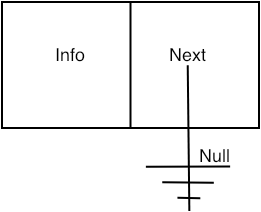
\includegraphics[scale=.3]{linkednode}
  \hfill
  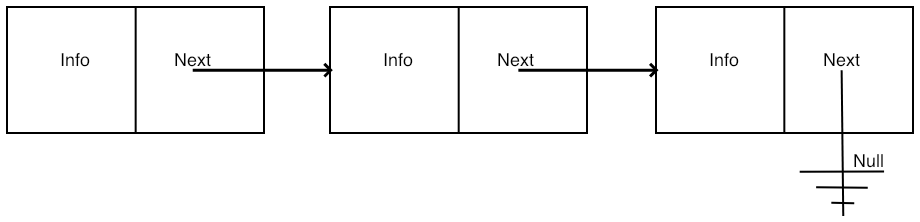
\includegraphics[scale=.3]{linkedlist}%
  }
  \caption{Node data structure and linked list of nodes}
  \label{fig:linked-node-list}
\end{figure}

If you need to do lots of insertions, make a
\emph{linked list}. The basic data structure is a \lstinline{Node},
which contains 
\begin{enumerate}
\item
  Information, which can be anything; and
\item A pointer (sometimes called `link') to the next node. If there
  is no next node, the pointer will be
  \emph{null}\index{pointer!null}. Every language has its own way of
  denoting a \indextermsub{null}{pointer}; C++~has the
  \indexc{nullptr}, while C~uses the \indexc{NULL} which is
  no more than a synonym for the value zero.
\end{enumerate}

We illustrate this in figure~\ref{fig:linked-node-list}.

\begin{slide}{Linked list structures}
  \label{sl:linkedlist}
  Linked list: data structure with easy insertion and deletion of
  information.

  Two basic elements:
  \begin{itemize}
  \item List, has pointer to first element, or null pointer
  \item Node, has information, plus pointer to next element (or null)
  \end{itemize}
  We are going to look at info routines about a list (`length'), or
  routines that alter the list (`insert').
\end{slide}
\begin{slide}{(in pictures)}
  \label{sl:linkedlist-pic}
  Node data structure and linked list of nodes
  
\hbox to \hsize{%
  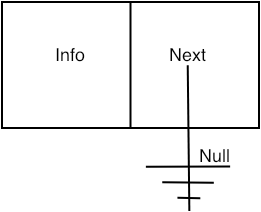
\includegraphics[scale=.2]{linkednode}
  \hfill
  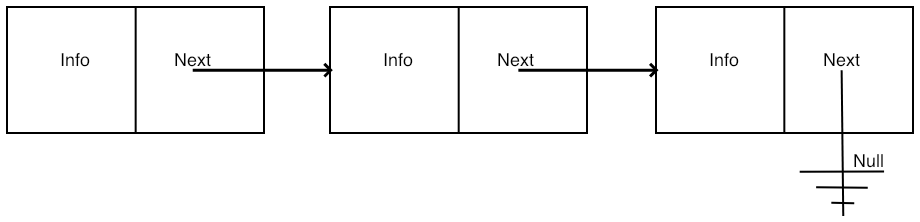
\includegraphics[scale=.2]{linkedlist}%
  }
\end{slide}

\begin{figure}[ht]
  \hbox to \hsize{%
  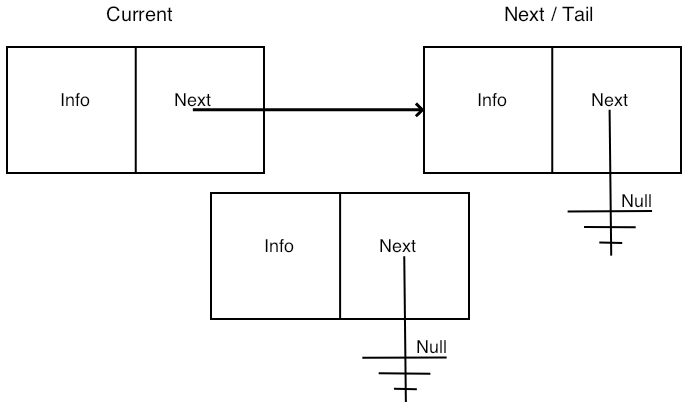
\includegraphics[scale=.3]{linkedinsert1}
  \hfill
  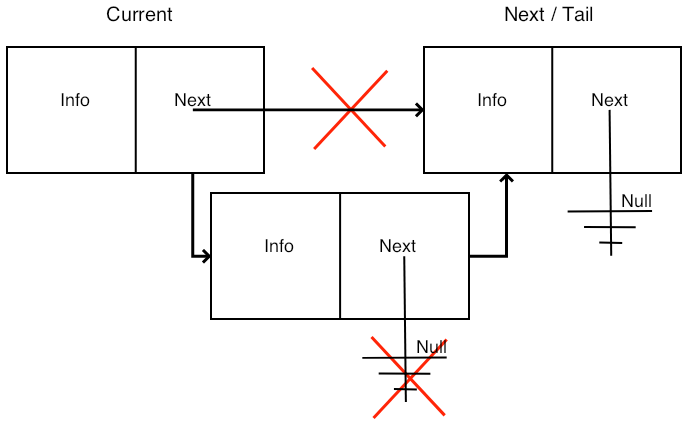
\includegraphics[scale=.3]{linkedinsert2}%
  }
  \caption{Insertion in a linked list}
  \label{fig:linked-list-insert}
\end{figure}

Our main concern will be to implement operations that report some
statistic of the list, such as its length, that test for the presence
of information in the list, or that alter the list, for
instance by inserting a new node. See figure~\ref{fig:linked-list-insert}.

\Level 2 {Data definitions}

In C++ you have a choice of pointer types. For now, we will use
\indexc{shared_ptr} throughout; later we will redo our code
using \indexc{unique_ptr}.

We declare the basic classes.
First we declare the \lstinline{List} class,
which has a pointer that is null for an empty list,
and pointing to the first node otherwise.

\begin{block}{Definition of List class}
  \label{sl:list-class}
  A linked list has as its only member a pointer to a node:
  %
  \verbatimsnippet{linklist}
  %
  Initially null for empty list.
\end{block}

Next, a \lstinline{Node} has an information field, which we here choose to be an integer,
and a counter to record how often a certain number has appeared.
The Node also has a pointer to the next node.
This pointer is again null for the last node
in the list.

\begin{block}{Definition of Node class}
  \label{sl:node-class}
  A~node has information fields, and a
  link to another node:
  %
  \lstset{numbers=left,numberstyle=\tiny}
  \verbatimsnippet{linknodeshared}
  %
  A Null pointer indicates the tail of the list.
\end{block}

We are now going to develop methods for the \lstinline{List} and \lstinline{Node}
classes that support the following code.

\begin{block}{List methods}
  \label{sl:list-node-funcs}
  List testing and modification.
\begin{lstlisting}
  List mylist;
  cout << "Empty list has length: "
       << mylist.length() << '\n';

  mylist.insert(3);
  cout << "After one insertion the length is: "
       << mylist.length() << '\n';
  if (mylist.contains_value(3))
    cout << "Indeed: contains 3" << '\n';
\end{lstlisting}
\end{block}

Let's start with some simple functions.

\Level 2 {Simple functions}

For many algorithms we have the choice between an iterative and a
recursive version. The recursive version is easier to formulate, but
the iterative solution is probably more efficient.

We start with a simple utility function for printing a linked list.
(This function is somewhat crude; a~better solution uses
the strategy from section~\ref{sec:lessless}.)
This implementation illustrates the recursive strategy.

\begin{block}{Print a list}
  \label{sl:linkedlist-print}
  Auxiliary function so that we can trace what we are doing.
  \begin{multicols}{2}
    Print the list head:
    \verbatimsnippet{listprint}
    \columnbreak
    Print a node and its tail:
    \verbatimsnippet{nodeprint}
  \end{multicols}
\end{block}

For recursively computing the length of a list,
we adopt this same recursive scheme.

\begin{block}{Recursive length computation}
  \label{sl:linkedlist-length-recur}
  For the list:
  \verbatimsnippet{listlengthrecursive}
  For a node:
  \verbatimsnippet{nodelengthrecursive}
\end{block}

An iterative version uses a pointer that goes down the list,
incrementing a counter at every step. 

\begin{block}{Iterative computation of the list length}
  \label{sl:linkedlist-length-iter}
  Use a shared pointer to go down the list:
  %
  \verbatimsnippet{listlengthiterative}
  (Fun exercise: can do an iterative de-allocate of the list?)
\end{block}

\begin{exercise}
  \label{ex:list-contains}
  Write a function
\begin{lstlisting}
bool List::contains_value(int v);
\end{lstlisting}
to test whether a value is present in the list.

This can be done recursive and iterative.
\end{exercise}

\Level 2 {Modification functions}

The interesting methods are of course those that alter the
list. Inserting a new value in the list has basically two cases:
\begin{enumerate}
\item If the list is empty, create a new node, and set the head of the
  list to that node.
\item If the list is not empty, we have several more cases, depending
  on whether the value goes at the head of the list, the tail,
  somewhere in the middle. And we need to check whether the value is
  already in the list.
\end{enumerate}
%% Our choice of using unique pointers dictates a certain design.

\begin{block}{Insert routine design}
  \label{sl:linklist-insert-proto}
  We will write functions
\begin{lstlisting}
void List::insert(int value);
void Node::insert(int value);
\end{lstlisting}
that add the value to the list.
The \lstinline{List::insert} value can put a new node in front of the first one;
the \lstinline{Node::insert} assumes that the value is great equal that of the current node.
\end{block}

There are a lot of cases here. You can try this by an approach called
\acf{TDD}: first you decide on a test, then you write the code that
covers that case.

%% \heading{Step 1: dealing with an empty list}

%% We start with an empty list, that is,
%% a head \lstinline{List} node that does
%% not point to any \lstinline{Node} nodes.

%% 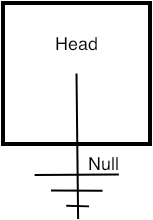
\includegraphics[scale=.3]{headempty}

%% \begin{exercise}
%%   Write a \lstinline{List::length} method, so that this code gives the right
%%   output:
%%   %
%%   \verbatimsnippet{liststep1}
%% \end{exercise}

\heading{Step 1: insert the first element}

Adding a first element to an empty list is simple:
we need the pointer of the head node
to point to a \lstinline{Node}.

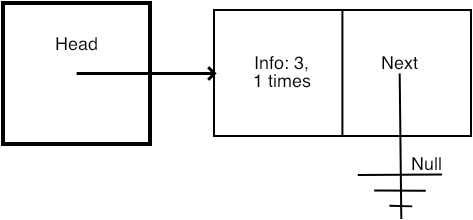
\includegraphics[scale=.3]{head3}

\begin{exercise}
  \label{ex:listlist-insert-empty}
  Next write the case of \lstinline{Node::insert} that handles the empty
  list. You also need a method \lstinline{List::contains} that tests if an
  item if in the list.
  %
  \verbatimsnippet{liststep2}
\end{exercise}

\heading{Step 3: inserting an element that already exists}

If we try to add a value to a list that is already there,
inserting does not do anything;
if needed we can increment a counter in the 
\lstinline{Node} that contains that value.

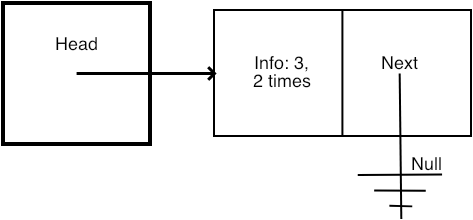
\includegraphics[scale=.3]{head33}

\begin{exercise}
  \label{ex:linklist-insert-already}
  Inserting a value that is already in the list means that the
  \lstinline{count} value of a node needs to be increased. Update your
  \lstinline{insert} method to make this code work:
  %
  \verbatimsnippet{liststep3}
\end{exercise}

\heading{Step 4: inserting an element at the head}
\par

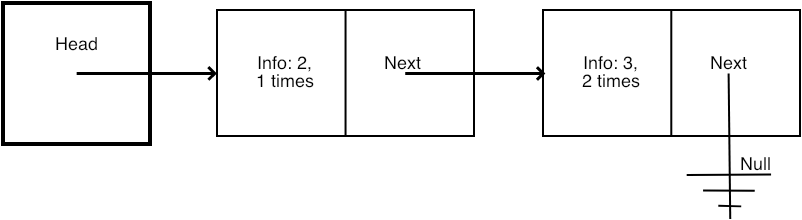
\includegraphics[scale=.3]{head23}

\begin{exercise}
  \label{ex:linklist-insert-head}
  One of the cases for inserting concerns an element that goes at the
  head. Update your \lstinline{insert} method to get this to work:
  %
  \verbatimsnippet{liststep4}
\end{exercise}

\heading{Step 5: inserting an element at the end}
\par

Adding an element to the tail requires traversing the whole list.

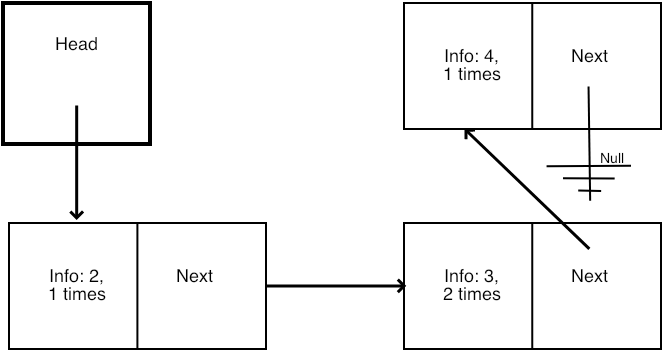
\includegraphics[scale=.3]{head234}

\begin{exercise}
  \label{ex:linklist-insert-tail}
  If an item goes at the end of the list:
  %
  \verbatimsnippet{liststep5}
\end{exercise}

\heading{Step 6: inserting an element in the middle}
\par

The trickiest case is inserting an element somewhere in the middle of the list.
Now you need to compare the current and next element to decide whether to
place the element or to move on to the tail.

\begin{block}{Insertion}
  \label{sl:linklist-insert-middle}
  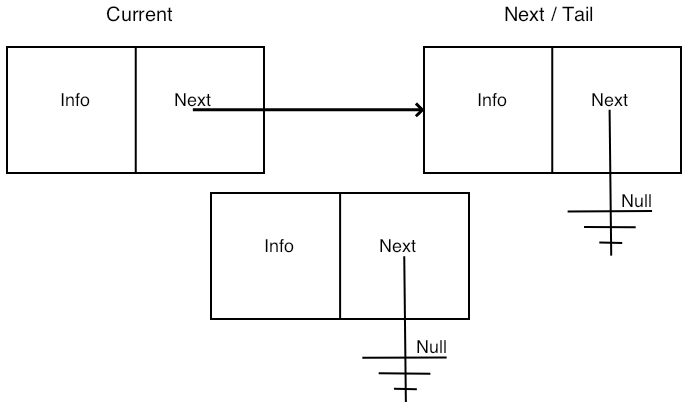
\includegraphics[scale=.25]{linkedinsert1}

  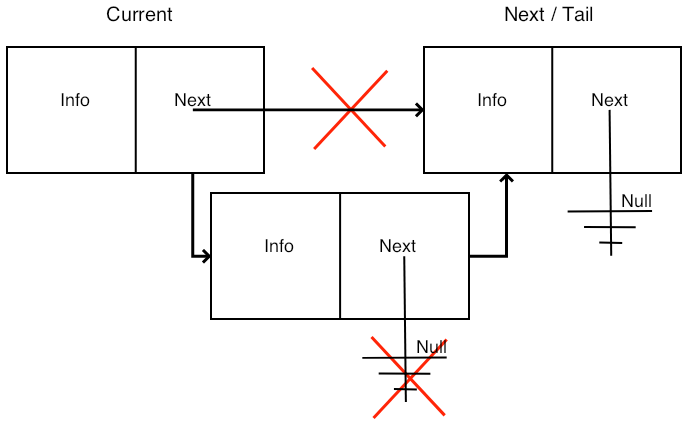
\includegraphics[scale=.25]{linkedinsert2}
\end{block}


\begin{exercise}
  \label{ex:linklist-insert-middle}
  Update your insert routine to deal with elements
  that need to go somewhere in the middle.
  
  \verbatimsnippet{liststep6}
\end{exercise}

\index{list!linked|)}

\Level 2 {Advanced: With unique pointers}

Conceptually we can say
that the list object owns the first node, and each node owns the
next.
Therefore, the most appropriate pointer type is  the \indexc{unique_ptr}.

We can also do this with unique pointers:

\begin{block}{Definition of List class}
  \label{sl:list-class-u}
  A linked list has as its only member a pointer to a node:
  %
  \lstset{numbers=left,numberstyle=\tiny}
  \verbatimsnippet{ulinklist}
  %
  Initially null for empty list.
\end{block}

\begin{block}{Definition of Node class}
  \label{sl:node-class-u}
  A~node has information fields, and a
  link to another node:
  %
  \lstset{numbers=left,numberstyle=\tiny}
  \verbatimsnippet{ulinknode}
  %
  A Null pointer indicates the tail of the list.
\end{block}

Above we formulated an iterative and a recursive way of computing
the length of a list.
The iterative code had a shared pointer pointing at successive
list elements. We can not do this with unique pointers.
Instead, this is a good place to use a \indextermsub{bare}{pointer}.

\begin{block}{Iterative computation of the list length}
  \label{sl:linkedlist-length-iter-u}
  Use a
  \indextermsub{bare}{pointer}, which is appropriate here because it doesn't
  own the node.
  %
  \verbatimsnippet{nodelengthiterativebare}
  %
  (You will get a compiler error if you try to make \lstinline{walker}
  a smart pointer: you can not copy a unique pointer.)
\end{block}

\begin{block}{Iterative vs bare pointers}
  \label{sl:bare-vs-smart}
  \begin{itemize}
  \item Use smart pointers for ownership
  \item Use bare pointers for pointing but not owning.
  \item This is an efficiency argument.\slidebreak
    I'm not totally convinced.
  \end{itemize}
\end{block}

\Level 1 {Trees}
\index{tree|(}
\prerequisite{ch:pointer}

A tree can be defined recursively:
\begin{itemize}
\item A tree is empty, or
\item a tree is a node with some number of children trees.
\end{itemize}
Let's design a tree that stores and counts integers: each node has a
label, namely an integer, and a count value that records how often we
have seen that integer.

Our basic data structure is the node, and we define it recursively to
have up to two children. This is a problem: you can not write
\begin{lstlisting}
class Node {
private:
  Node left,right;
}
\end{lstlisting}
because that would recursively need infinite memory. So instead we use pointers.
%
\verbatimsnippet{treenode}
%
and we record that we have seen the integer zero zero times.

Algorithms on a tree are typically recursive. For instance, the total
number of nodes is computed from the root. At any given node, the
number of nodes of that attached subtree is one plus the number of
nodes of the left and right subtrees.
%
\verbatimsnippet{treecount}

Likewise, the depth of a tree is computed as a recursive max over the
left and right subtrees:
%
\verbatimsnippet{treedepth}

Now we need to consider how actually to insert nodes. We write a
function that inserts an item at a node. If the key of that node is
the item, we increase the value of the counter. Otherwise we determine
whether to add the item in the left or right subtree. If no such
subtree exists, we create it; otherwise we descend in the appropriate
subtree, and do a recursive insert call.
%
\verbatimsnippet{treeinsert}

%%packtsnippet end

\index{tree|)}

\Level 1 {Other graphs}

The nodes in a tree have a relation from parent-to-child, so
they are a special case of a \indextermsub{directed}{graph}.

\begin{exercise}
  If you know about the relationship between graphs and their
  \indextermsub{adjacency}{matrix},
  can you express directedness in terms of matrix properties?
\end{exercise}

An important subset or directed graphs, that of \acp{DAG},
has a property that trees do not have:
for some pairs of nodes they may have more than one
path between them.

For more details, see~\HPSCref[chapter]{app:graph}.

\Level 0 {Algorithms}

This \emph{really} \textbf{really} goes beyond this book.

\begin{itemize}
\item Simple ones: numerical
\item Connected to a data structure: search
\end{itemize}

\Level 1 {Sorting}

Unlike the tree algorithms above, which used a non-obvious data
structure,
sorting algorithms are a good example of the combination of very
simple data structures (mostly just an array), and sophisticated
analysis of the algorithm behavior. We very briefly discuss two
algorithms.

The standard library has a sorting routine built-in;
see section~\ref{sec:stl:sort}.

\Level 2 {Bubble sort}

An array $a$ of length~$n$ is sorted if
\[ \forall_{i<n-1}\colon a_i\leq a_{i+1}. \]
A simple sorting algorithm suggests itself immediately: if $i$ is such
that $a_i>a_{i+1}$, then reverse the $i$ and $i+1$ locations in the
array.

\verbatimsnippet{swaplocs}

(Why is the array argument passed by reference?)

If you go through the array once, swapping elements, the result is not
sorted, but at least the largest element is at the end. You can now do
another pass, putting the next-largest element in place, and so on.

This algorithm is known as \indexterm{bubble sort}. It is generally
not considered a good algorithm, because it has a time complexity
(section~\ref{sec:time_complex}) of $n^2/2$ swap operations. Sorting
can be shown to need $O(n\log n)$ operations, and bubble sort is far
above this limit.

\Level 2 {Quicksort}

A popular algorithm that can attain the optimal complexity (but need
not; see below) is \indexterm{quicksort}:
\begin{itemize}
\item Find an element, called the pivot, that is approximately equal
  to the median value.
\item Rearrange the array elements to give three sets, consecutively
  stored: all elements less than, equal, and greater than the pivot
  respectively.
\item Apply the quicksort algorithm to the first and third subarrays.
\end{itemize}

This algorithm is best programmed recursively, and you can even make a
case for its parallel execution: every time you find a pivot you can
double the number of active processors.

\begin{exercise}
  Suppose that, by bad luck, your pivot turns out to be the smallest
  array element every time. What is the time complexity of the
  resulting algorithm?
\end{exercise}

\Level 1 {Graph algorithms}

We briefly discuss some graph algorithms.
For further discussion see~\HPSCref[chapter]{app:graphalgorithms}.

First consider the \ac{SSSP} problem:
given a graph and a starting node,
what is the shorted path to every other node.
Initially, we consider an \indextermsub{unweighted}{graph},
or equivalently, set the distance between any pair of connected
nodes to~1.

The algorithm proceeds by levels: each next level consists of
the neighbors of already explored nodes.

\begin{itemize}
\item Set the distance to the starting node to zero.
\item Until done,
\item Loop over all nodes with known distance, and
\item for all of its neighbors,
  \begin{itemize}
  \item unless the neighbor already has a known distance
  \item set the distances to~$d+1$,
  \end{itemize}
\end{itemize}

We use a simple data structure for the distances:
\begin{lstlisting}
map<int,int> distances;  
int starting_node = 0;
distances[starting_node] = 0;
\end{lstlisting}

Until all nodes are mapped,
we iterate over nodes for which the distances are know, 
and set the distance for their neighbors:

\begin{lstlisting}
// while not done
for (;;) {
  int updates{0};
  // iterate over all mapped nodes
  for ( auto [node,dist] : distances ) {
    // for each, iterate over all of their neighbors
    }
  }
}  
\end{lstlisting}

Assume that the graph data structure supports
getting the list of neighbors of a node:
\begin{lstlisting}
for ( const auto& neighbor : graph.neighbors(node) ) {
  if ( auto find_neighbor = distances.find(neighbor) ; find_neighbor==distances.end() ) {
      distances[neighbor] = dist+1; updates++;
  }
}
\end{lstlisting}

Since we use a until-done loop, we need to break out of explicitly.
A~simple test would be `if the number of mapped nodes equals the number
of nodes in the graph'.

\begin{exercise}
  Can you see a problem with this, and a way to fix it?
\end{exercise}

The above algorithm is a little wasteful:
in each pass it traverses all mapped nodes,
but we only need the newly added ones.
Therefore we add:
\begin{lstlisting}
set<int> current_front;
current_front.insert(starting_node);
for (;;) {  
  set<int> next_front;
  // iterate over current_front
  for ( auto node : current_front ) {
    // iterate over neighbors
    for ( const auto& neighbor : graph.neighbors(node) ) {
      // if neighbor not yet mapped
	if ( /* ... */ ) {
          distances[neighbor] = dist_to_this_node+1;
          next_front.insert(neighbor);
        }
    }
  }
  current_front = next_front;
}
\end{lstlisting}

\Level 0 {Programming techniques}

\Level 1 {Memoization}
\label{sec:memo}

In section~\ref{sec:recursion} you saw some examples of recursion. The
factorial example could be written in a loop, and there are both arguments
for and against doing so. 

The Fibonacci example is more subtle: it can not immediately be
converted to an iterative formulation, but there is a clear need for
eliminating some waste that comes with the simple recursive
formulation. The technique we can use for this is known as
\indextermdef{memoization}: store intermediate results to prevent them
from being recomputed.

Here is an outline.
\verbatimsnippet{fibomemo}
